\chapter{Avaliação}
\label{c_avaliacao}
Este capítulo apresenta o contexto de realização da pesquisa e os procedimentos metodológicos adotados. Esta pesquisa tem abordagem qualitativa exploratória, buscando gerar dados descritivos e explanatórios, em vez de demonstrar estatisticamente relações de causa e efeito. Além disso, a pesquisa foi participante, caracterizada por atuação ativa do pesquisador nas atividades. 

O objetivo foi observar e descrever as interações das crianças com a RoPE AR durante a programação e depuração de algoritmos. Para isso, a \autoref{sec:contexto} descreve o contexto de realização da pesquisa e a \autoref{sec:participantes} descreve os participantes. Por fim, a \autoref{sec:protocolo} apresenta os experimentos realizados, detalhando a estratégia de coleta de dados e o método de análise destes dados.

\section{Contexto}
\label{sec:contexto}
\subsection{Município}
A coleta de dados ocorreu em um \ac{CDI} no município de Gaspar, no estado de Santa Catarina. A respeito da cidade, O IBGE (Instituto Brasileiro de Geografia e Estatística) estima a população em 70.793 pessoas, com uma densidade demográfica de 150 pessoas por km\textsuperscript{2}. Aproximadamente 40\% da população tem ocupação, sendo que o salário médio dos trabalhadores formais é 2,4 salários-mínimos. O índice de desenvolvimento humano é 0,765, e está acima da média nacional de \. A taxa de mortalidade infantil é 4,42 a cada 1000 nascidos vivos, contra \ no Brasil. A taxa de escolarização entre 6 e 14 anos é de 97,3\%.
\subsection{Centro de Desenvolvimento Infantil}
\label{sec:cdi}
A pesquisa ocorreu em um  \ac{CDI} de um bairro urbano de Gaspar, distante aproximadamente cinco quilômetros do centro da cidade. O local foi selecionado por conveniência, pois o pesquisador conhece uma professora que leciona no local, o que possibilitou a execução de pesquisas em anos anteriores. A pesquisa atual, entretanto, não ocorreu nas turmas desta professora. Além disso, nenhum dos participantes conhecia o brinquedo RoPE. Outro critério para a seleção do centro foi a presença de internet, pois projetor disponível utiliza conexão sem fio local.

O \ac{PPP} do \ac{CDI} apresenta dados históricos e da estrutura física do local. O mesmo foi fundado em 1990, sendo uma parceria entre a prefeitura municipal e a associação de moradores do bairro. Atualmente possui 38 colaboradores, que promovem o atendimento de 246 crianças. A idade atendida vai de zero e cinco anos e onze meses, e há 12 turmas organizadas em três grupos etários: Infância I (0 a 2 anos), Infância II (2 a 4 anos) e Infância III (4 a 6 anos). Dentro de cada grupo etário as turmas também são divididas. Na Infância III, por exemplo, há as turmas de 4 a 5 e de 5 a 6 anos. O espaço tem 9 salas onde as professoras realizam suas atividades, uma biblioteca com aproximadamente 300 livros infantis, um parquinho, banheiros, sala de coordenação e sala do zelador. Além das salas existentes, está em curso a construção de novos espaços no local onde antes havia o parquinho, o qual foi deslocado para um espaço ao lado do CDI. 

O \ac{PPP} do \ac{CDI} apresenta um diagnóstico da comunidade, construído a partir de um questionário. O trabalho apresenta gráficos de pizza, que serão analisados visualmente pois não apresentam dados numericamente (\autoref{fig:contexto_ppp}). Aproximadamente 2/3 das crianças mora com pai e mãe, metade vai de carro ao \ac{CDI}, e quase a metade não tem computador em casa. A respeito dos pais, a maior parte auxilia os filhos nas atividades do \ac{CDI} mas não tem disponibilidade em horário comercial. A renda de aproximadamente a metade das famílias é de 1 a 2 salários-mínimos, e de outra metade vai de 2 a 4.

\begin{figure}[!htbp]
    \centering
    \begin{subfigure}{.3\linewidth}
        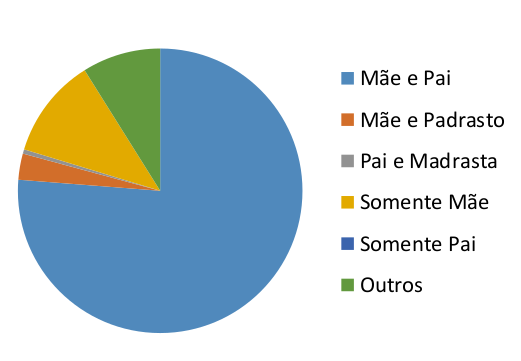
\includegraphics[width=.9\linewidth,fbox]{figs/cdi/mora_com.png}
        \caption{Com quem a criança mora.}
        \label{fig:mora_com}
    \end{subfigure}%
    \begin{subfigure}{.3\textwidth}
        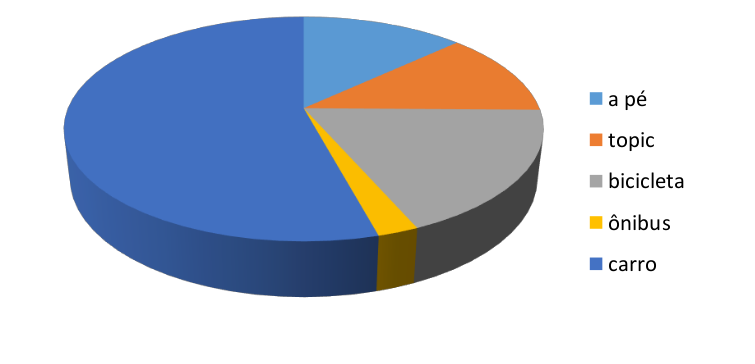
\includegraphics[width=.9\linewidth,fbox]{figs/cdi/meio_transporte.png}
        \caption{Meio de transporte.}
        \label{fig:transporte}
    \end{subfigure}%
   \begin{subfigure}{.3\textwidth}
        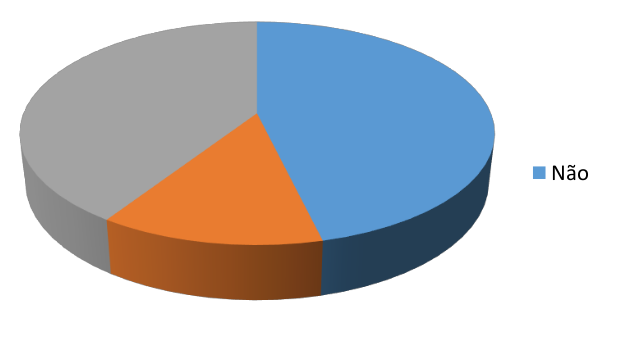
\includegraphics[width=.9\linewidth,fbox]{figs/cdi/tem_computador.png}
        \caption{Tem computador em casa?}
        \label{fig:tem_computador}
    \end{subfigure}
    \begin{subfigure}{.3\textwidth}
        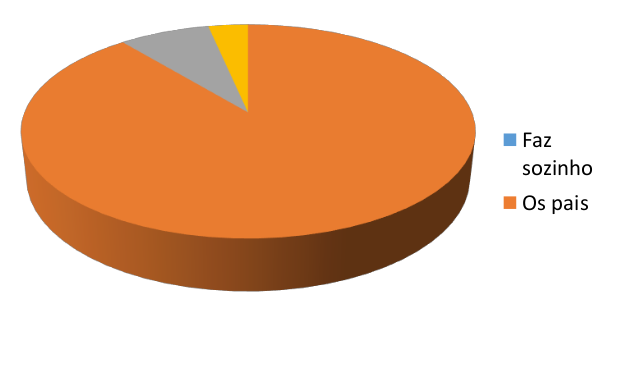
\includegraphics[width=.9\linewidth,fbox]{figs/cdi/pai_auxilia_crianca_atividades.png}
        \caption{Auxílio dos pais nas atividades do CDI}
        \label{fig:pai_auxilia_crianca_atividades}
    \end{subfigure}%
    \begin{subfigure}{.3\textwidth}
        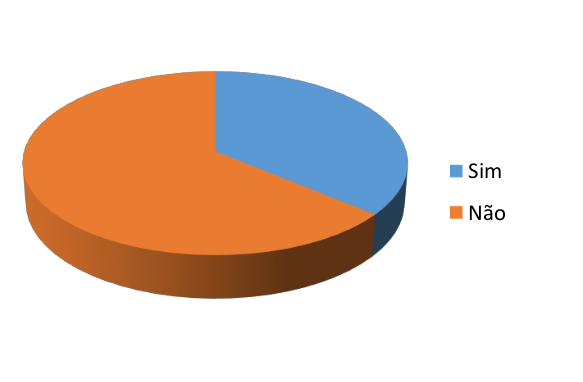
\includegraphics[width=.9\linewidth,fbox]{figs/cdi/disponibilidade_pais_horario_comercial.png}
        \caption{Disponibilidade dos pais em horário comercial.}
        \label{fig:disponibilidade_pais_horario_comercial}
    \end{subfigure}%
     \begin{subfigure}{.3\textwidth}
        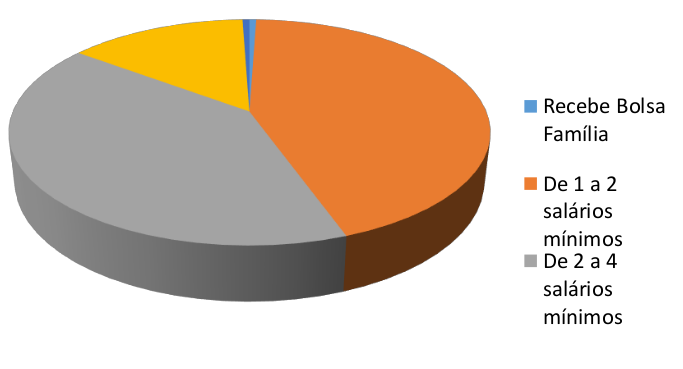
\includegraphics[width=.9\linewidth,fbox]{figs/cdi/renda.png}
        \caption{Renda mensal familiar.}
        \label{fig:renda}
    \end{subfigure}%
    \caption{Dados do Projeto Político Pedagógico do CDI.}
    \label{fig:contexto_ppp}
\end{figure}
Considerando os dados do IBGE e do PPP, infere-se que as condições de vida na região não são precárias, porém a necessidade de trabalho impede o acompanhamento dos filhos em horário comercial. Em horário compatível, porém, os pais buscam auxiliar os filhos nas atividades.

\subsection{Proposta Pedagógica para a Educação Infantil}
Mesmo com as suas particularidades locais, todos os CDIs de Gaspar buscam seguir uma mesma proposta pedagógica alinhada com a rede de ensino do municipal. O documento orientador é a Proposta Pedagógica da Rede Municipal para a Educação Infantil \cite{gaspar_proposta_2010}. Essa proposta foi publicada em 2010, após ser construída coletivamente pelos professores e professoras da Rede Municipal de Educação Infantil. O resultado é um documento que busca nortear o trabalho pedagógico “para e com” as crianças pequenas.

Este “norte” tem duas bases principais: os eixos de Linguagens, Interações e Brincadeiras, e a abordagem metodológica de projetos. Quanto aos eixos, o eixo de Linguagens tem como objetivo incrementar as aprendizagens infantis por meio de atividades que envolvam uso do corpo (linguagem motora); exploração dos sons (linguagem musical); exploração de cores, formas e texturas (linguagem plástica); fala e códigos (linguagem oral e escrita) e noções de espaço, quantidade e números (linguagem matemática). O eixo de Interações diz respeito ao planejamento e organização de situações de contato entre criança-criança, criança-adulto e criança-objeto. Por fim, o eixo das brincadeiras busca aumentar o repertório de interações lúdicas entre as crianças, orientando o educador a observar, coordenar ou integrar-se nas brincadeiras.

Já a Metodologia de Projetos, segundo a proposta, é uma abordagem que permite combinar as intenções pedagógicas do adulto e também estimular a curiosidade da criança. Esse estímulo se dá ao propor projetos em que há investigação de algum tema ou construção de algo com foco em assuntos do mundo infantil (ver \autoref{fig:tres_porquinhos}). Os temas dos projetos surgem em diálogos durante rodas de conversa, passeios ou brincadeiras. Partindo do interesse das crianças, os projetos seguem uma estrutura com hipóteses, perguntas de pesquisa, descrições e comparações. Não há prazo de início e fim, e também não há necessidade de trabalhar diariamente com projetos. Quando nenhum projeto está em curso, trabalha-se seguindo os eixos de Linguagens, Interações e Brincadeiras.

\begin{figure}[!h]
    \centering
    \begin{subfigure}{.45\linewidth}
        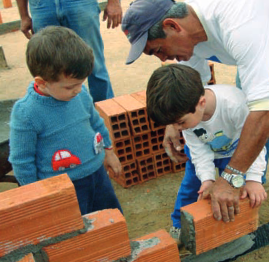
\includegraphics[width=.8\linewidth,fbox]{figs/tres_porquinhos.png}
        \caption{Projeto de construção de casa de tijolos (História dos Três Porquinhos).}
        \source{Proposta Pedagógica da Rede Municipal de Educação Infantil de Gaspar (2010). }
        \label{fig:tres_porquinhos}
    \end{subfigure}%
    \hspace{.05\textwidth}%
    \begin{subfigure}{.45\textwidth}
        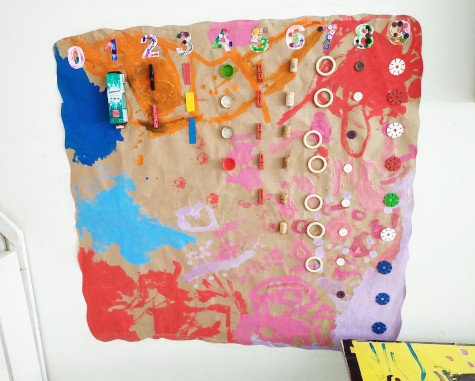
\includegraphics[width=.8\linewidth,fbox]{figs/projeto_numeros_menor.jpeg}
        \caption{Projeto para assimilação de quantidades. Turma de 4 a 5 anos.}
        \source{O autor.}
        \label{fig:projeto_numeros}
    \end{subfigure}%
\end{figure}
A proposta não menciona diretamente o tema das tecnologias digitais. Palavras como \textit{celular} e \textit{computador} não são citadas. Ainda assim, a relação com o “mundo digital” é aderente aos eixos e abordagens metodológicas propostas. As Interações, por exemplo, podem ser favorecidas pelo RoPE AR, quando a criança aperta botões e encaixa blocos que provocam reações em um objeto. Há também o uso de uma Linguagem para comunicar uma sequência de ações à um objeto (o brinquedo RoPE). Por fim, a atividade em si é uma Brincadeira, que segundo a proposta deve envolver elementos acolhedores, desafiadores e inclusivos \cite[p.50]{gaspar_proposta_2010}. 

% restaurante, canto caverna, castelo das bonecas, área de animais aquáticos, robô

\section{Participantes da pesquisa}
\label{sec:participantes}
Apresentado o contexto do local da pesquisa e a proposta pedagógica adotada, é preciso comentar sobre os participantes. Participaram 26 crianças com idades entre 4 e 6 anos, frequentadoras de um CDI público de um bairro de Gaspar. Entretanto, a análise considera a participação de 20 crianças, devido ao descarte de vídeos inadequados\footnote{O posicionamento da câmera impediu ver as ações das crianças ou mais de três crianças interagiram simultâneamente com o brinquedo, sem que o pesquisador conseguisse estruturar a a atividade.}.

As crianças e as professoras estiveram distribuídos em três salas. A primeira sala (5-6A) atende crianças entre 5 e 6 anos, e as outras duas salas (4-5A e 4-5B) atendem crianças entre 4 e 5 anos. Cada sala recebe crianças diferentes no período matutino e vespertino. Além disso, as crianças alternam as aulas no CDI e em casa a cada semana, devido à necessidade de distanciamento social.

No primeiro dia a atividade ocorreu na sala de 5 a 6 anos, no período vespertino. No segundo dia a visita ocorreu na segunda sala durante o período vespertino, com crianças de 4 a 5 anos. Por fim, no quarto dia a terceira sala visitada foi a da segunda turma de 4 a 5 anos, tanto de manhã quanto à tarde. Ao fim, quatro grupos de crianças participaram (\autoref{quadro:participants}):

 \begin{quadro}[!h]
 		\setlength{\extrarowheight}{3pt}
        \begin{center}
        \caption{Encontros e participantes}
        \label{quadro:participants}
        \begin{tabular}{@{}llcccc@{}}
            \toprule
            Grupo & Encontro & Turma  & Meninas & Meninos & Professoras \\ \midrule
            1         & Dia 1                       & 5 a 6 anos - Tarde      & 3 & 2 & Daiana e Maria \\
            2         & Dia 2                       & 4 a 5 anos A - Tarde   & 0 & 3 & Paula e Joana \\
            3         & Dia 3                       & 4 a 5 anos B - Manhã & 4 & 2 & Vera e Lúcia \\
            4         & Dia 3                       & 4 a 5 anos B - Tarde   & 2 & 4 & Vera e Lúcia \\ \midrule
            4 grupos          & 3 dias        & 5 turmas     & 9 & 11 & Seis professoras \\ \bottomrule 
            \end{tabular}
        \end{center}
        \sourceauthor
    \end{quadro}

Além das crianças, as professoras de cada uma das três salas também participaram. Cada sala possui uma professora e uma assistente, que serão tratadas aqui como professoras. Todas são mulheres, e possuem de 4 a 28 anos de experiência de trabalho com crianças. Das seis professoras participantes, três responderam diretamente a entrevistas e outras três colaboraram em algum momento por meio de comentários a respeito do projeto ou auxiliando na comunicação com as crianças. As nomes utilizados no texto são fictícios, a fim de evitar a identificação dos participantes
\footnote{
    O guia \textit{Orientações para relato de Pesquisa Qualitativa envolvendo Tecnologias Educacionais}, do \ac{CIEB}, sugere também descrever o pesquisador como um participante. O pesquisador é um sujeito que nunca está ausente, e suas vivências e experiências anteriores impactam a compreensão do fenômeno em estudo. O pesquisador do presente trabalho é um homem de 26 anos, com formação em computação e experiência em desenvolvimento de softwares para empresas. Em estudos anteriores na universidade desenvolveu interfaces para o brinquedo RoPE. Nessa experiência as crianças interagiram via aplicativo, e o pesquisador dificuldade das crianças usarem o smartphone, pois que não conseguiam arrastar elementos na tela. No mesmo trabalho considerou o smartphone como um dispositivo inadequado para o ambiente de um CDI, pois havia o medo de que alguma criança o quebrasse. A interação das crianças apenas com elementos tangíveis seria uma alternativa a esses problemas, pois manipular objetos tangíveis é atividade rotineira nos CDIs. Essas experiências prévias podem representar viéses desta pesquisa e uma ameaça à validade dos resultados.
}.

O recrutamento, portanto, se deu por conveniência. As crianças participantes frequentavam o ambiente no dia da visita do pesquisador. Não houve distinção de sexo ou presença/ausência de deficiência intelectual. A ordem de participação das crianças se deu com o pesquisador solicitando à participação de crianças e as professoras selecionando as crianças. As crianças que quiseram participar antes da solicitação não foram impedidas. Deste modo não houve um controle rígido do acesso à interface, mas sim uma organização para evitar mais de três crianças utilizando ao mesmo tempo. Quanto às professoras, participaram das entrevistas as responsáveis pela turma em questão ou as que se sentiram confortáveis em responder.

\section{Ambiente}
As atividades ocorreram em três salas comumente frequentadas pelas crianças. Em todas as salas o projetor ficou em um suporte, posicionado ao lado de uma fonte de energia e afastado de janelas e portas. As luzes das salas foram apagadas, mas isso não modificou o ambiente a ponto de torná-lo escuro (ver \autoref{fig:setting}). No chão, à frente do projetor, foram fixadas duas cartolinas brancas para receber as imagens projetadas. Ao lado do projetor um notebook foi posicionado para servir como câmera. 

\begin{figure}[!h]
    \centering
    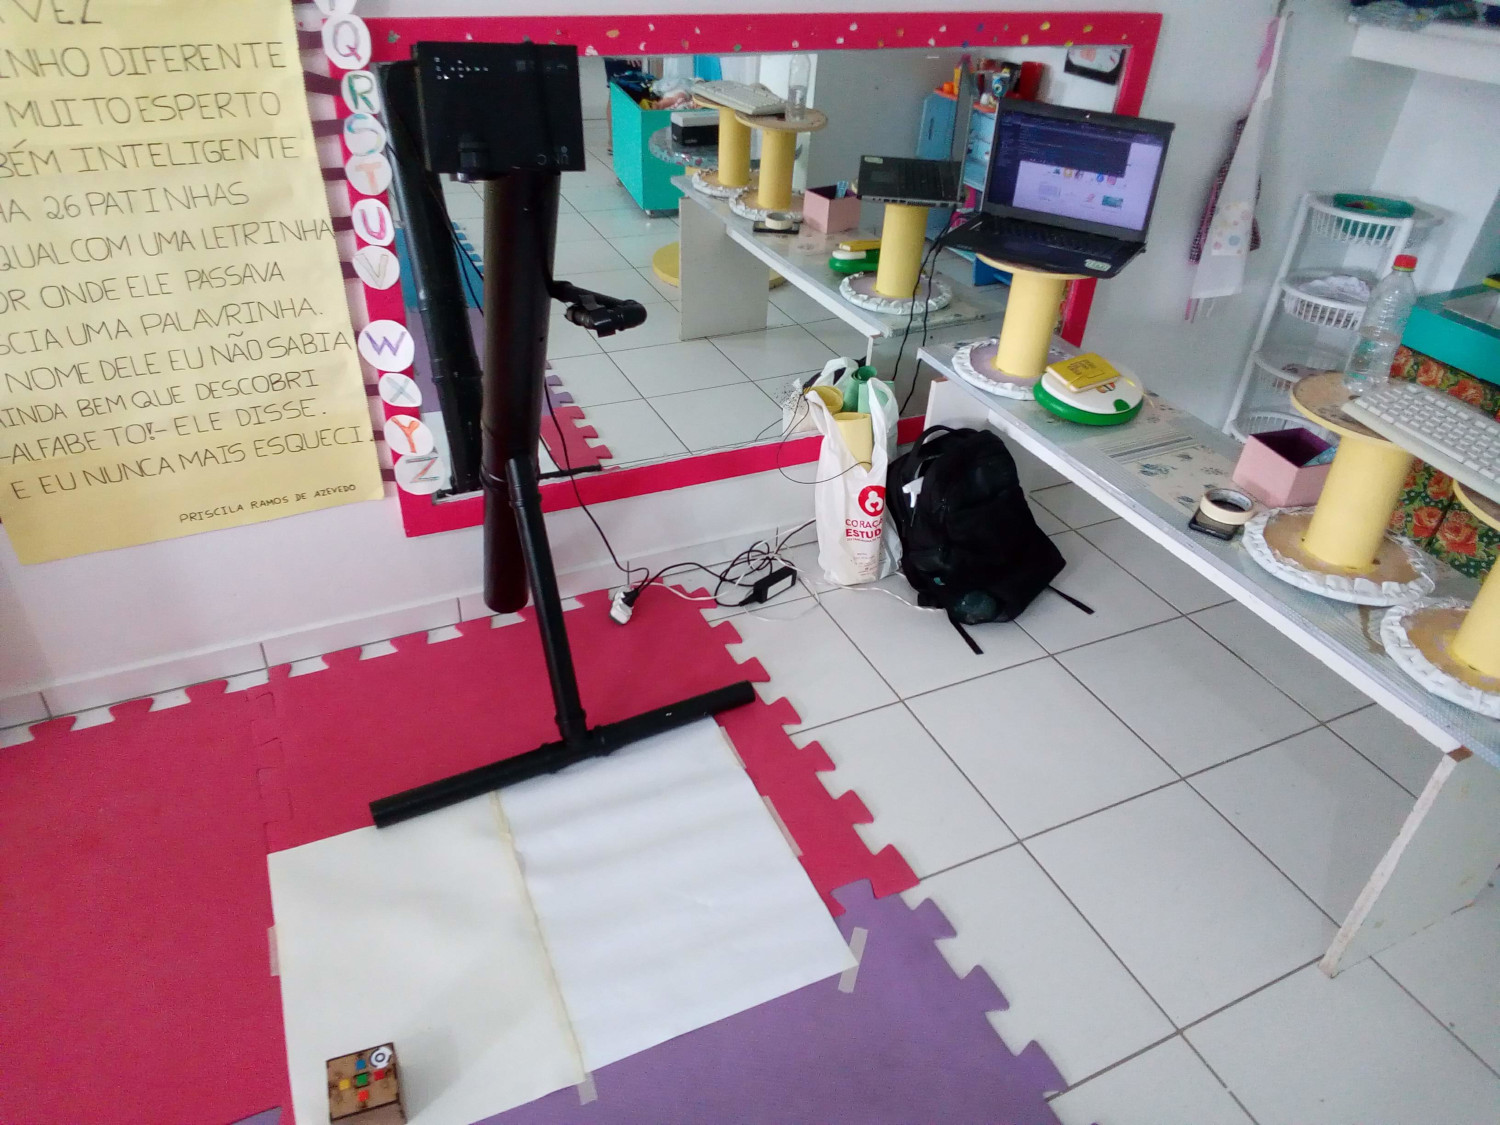
\includegraphics[width=0.8\textwidth,fbox]{figs/setting_projector.jpg}
    \caption{Posicionamento do projetor.}
    \label{fig:setting}
\end{figure}

As crianças continuaram suas atividades junto às professoras enquanto o pesquisador organizava os equipamentos. Era perceptível a curiosidade das crianças a respeito dos materiais e da figura do pesquisador, tanto pelos olhares quanto por perguntas feitas às professoras. Ao lado da sala da turma 4-5A há um espaço externo gramado. Neste ambiente a professora continuou as atividades no espaço externo, e a programação do RoPE ocorreu dentro da sala com a outra professora presente. As outras duas salas tem espaços amplos, e todas as crianças permaneceram no recinto durante a atividade. Enquanto duas ou três participavam da pesquisa, as demais continuavam suas atividades em uma outro ponto da sala.

O CDI tem rede de internet sem fio, porém a qualidade do sinal é variável em cada sala. Especificamente na sala 4-5A há dificuldade de manter a conexão. Esse problema foi mencionado pelas professoras e se ocorreu durante a conexão do projetor na rede. As demais salas visitadas, porém, tem conexão estável.

\section{Materiais e Protocolo de Coleta de Dados}
\label{sec:protocolo}
Após a organização do ambiente ocorreu o contato das crianças com a RoPE AR. Esse contato seguiu um roteiro base com cinco etapas. Apesar do roteiro, as atividades foram flexíveis para se adaptar ao contexto de sala de aula, às sugestões das crianças, dificuldades, curiosidades, e restrições de tempo existentes. 

O trecho a seguir descreve o protocolo seguido. Os rótulos [MAT] e [ETAPA] destacam os materiais e etapas do protocolo.

\relato{
    Após ajustar o projetor [MAT PROJETOR] no suporte [MAT SUPORTE] e iniciar a gravação com a câmera do notebook [MAT CÂMERA], o pesquisador perguntou quais crianças gostariam de iniciar a brincadeira. A professora perguntou quantas crianças poderiam participar por vez, e o pesquisador respondeu que o ideal seria um grupo de duas ou três crianças [ETAPA 1 - SELEÇÃO]. A professora então chamou duas crianças pelo nome, que interromperam suas atividades junto às demais e se dirigiram até o pesquisador.

    As duas crianças e o pesquisador se sentaram em um tapete, visível na câmera. Para ambientação [ETAPA 2 - AMBIENTAÇÃO], o pesquisador se apresentou e pediu para as crianças falarem seus nomes e idades. Depois disso apresentou a atividade: "Hoje nós vamos conhecer um robô. Vocês conhecem algum robô? Como ele é? O que ele faz?". Cada criança respondeu se conhecia ou não algum robô, geralmente mencionando brinquedos ou personagens de desenhos animados. Depois da conversa inicial, o pesquisador apresentou o RoPE [MAT ROPE] e os blocos de papelão [MAT BLOCOS]. Para cada bloco, perguntou [ETAPA 3 - COMPREENSÃO DOS SÍMBOLOS DOS BLOCOS]: "O que vocês estão vendo neste desenho aqui?". Em caso de resposta errada ou ausência de resposta, o pesquisador perguntou: "O que o robô está fazendo?". Também buscou observar como as crianças encaixavam os blocos, quais relacionamentos percebiam entre os blocos e os botões do brinquedo. A cada execução do robô, o smartphone enviou os comandos informados para a CtPuzzle Platform [MAT CONEXÃO COM A INTERNET].

    Após o reconhecimento dos blocos, o aplicativo [MAT SMARTPHONE] e a projeção foram ligados. O pesquisador perguntou o que as crianças viam na área projetada, e essas responderam que estavam vendo uma maçã. O pesquisador explicou às crianças que deveriam ajudar o RoPE pegar a maçã, andando pelo caminho marrom, e para isso deveriam usar os blocos [ETAPA 4 - PROGRAMAÇÃO]. Para a primeira maçã o pesquisador explicou o funcionamento: colocou o RoPE na posição inicial, encaixou o bloco Frente (azul) no bloco Início (verde) e apertou o botão verde (iniciar) do RoPE. O brinquedo andou para frente e capturou a maçã. As crianças programaram os o robô para pegar as próximas quatro maçãs. Dúvidas e erros ocorreram com frequência, e o pesquisador auxiliou fazendo perguntas e dando exemplos quando necessário, e explicando as regras e direções.
    
    Após a captura das 5 maçãs na primeira etapa, iniciou a etapa de depuração [ETAPA 5 - DEPURAÇÃO]. O pesquisador sequenciou os blocos de forma a haver um erro que faria o RoPE não pegar a maçã, e solicitou às crianças que tentassem encontrá-lo. Nos casos em que as crianças não encontraram o erro imediatamente, o pesquisador pediu para apertarem o botão verde, e ver o robô na direção errada, e então corrigirem o erro. Essa ação repetiu-se por  A brincadeira terminou quando todos os erros foram encontrados. O pesquisador agradeceu às crianças, e perguntou se a o vídeo da atividade poderia ser usada no seu trabalho. Para isso apresentou dois rostos em uma folha pequena, um alegre e um triste. As crianças consentiram no uso do vídeo pintando o rosto alegre [MAT FOLHA DE CONSENTIMENTO].
}

\begin{figure}[!ht]
    \centering
    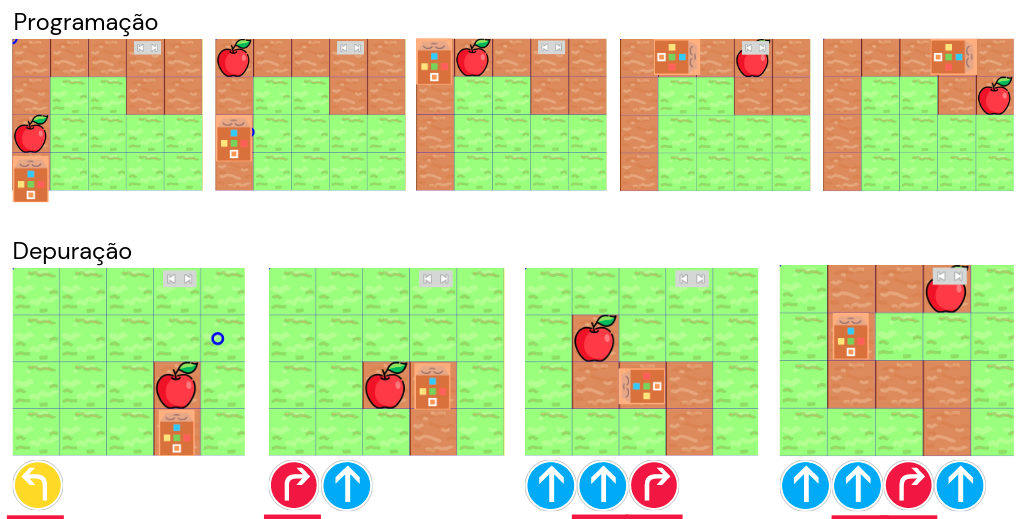
\includegraphics[width=.8\linewidth,fbox]{figs/phases.png}
    \caption{Problemas de programação e depuração apresentados durante a coleta de dados. }
    \sourceauthor
    \label{fig:phases}
\end{figure}

A \autoref{fig:phases} apresenta as cinco fases de programação e as quatro fases de depuração citadas no trecho a cima. As fases exigem um número crescente de passos para a resolução do problema. A primeira fase, por exemplo, necessita de apenas um movimento, enquanto a segunda necessita de dois. A terceira fase adiciona a necessidade do movimento de giro. O mesmo ocorre nas fases de depuração. Além disso, o pesquisador criou previamente um algoritmo com erro, destacado em vermelho na figura. A solução da primeira atividade de depuração seria um avanço à frente, porém o algoritmo criado tem um giro à esquerda. A atividade consiste, então, em discutir sobre o algoritmo e resolver o problema. Não foi exigida a finalização de todas as fases. Em casos onde se percebeu dificuldade em finalizar, com repetição de mesmos erros, ou quando se percebeu cansaço e distração das crianças, a tarefa foi interrompida de comum acordo entre e pesquisador e professoras.


\begin{comment}
\begin{itemize}
\item 
\item O que você vê neste desenho? O que está desenhado aqui?
\item Porque você acha que o RoPE está se movendo deste jeito?
\item Como você encaixaria esses desenhos?
\end{itemize}

%A força motriz do design iterativo são as metas do usuário, que são ações que o usuário deseja poder fazer \cite{rogers_design_2013}. Neste trabalho, o alcance das metas de usabilidade se dá quando a criança:

\begin{itemize}
    \item posiciona o brinquedo na posição inicial;
    \item percebe que os blocos representam ações do robô;
    \item sequencia blocos formando um algoritmo;
    \item inicia execução do algoritmo;
    \item altera sequência de blocos; e
    \item percebe blocos destacados durante execução.
\end{itemize}

Para direcionar a observação, as categorias de análise serão 
(i) para quais elementos da interface as crianças olham;
(ii) se e como as crianças manipulam os blocos; 
(iii) perguntas realizadas; 
(iv) se e como as crianças comparam os blocos com os símbolos do robô; 
(v) como ocorre o início da execução; 
(vi) em que local e direção posicionam o robô; e 
(vii) se e como os elementos virtuais são percebidos pelas crianças.

%A colaboração será observada quando duas ou mais crianças brincarem em conjunto com os blocos. Esse tipo de evento já foi observado em estudos anteriores \cite{sapounidis_tangible_2019, raabe_estudo_2019}, mas precisa ser confirmado neste estudo para afirmar que a interface apresentada tem os benefícios das interfaces tangíveis. 

% \cite{bardin_alise_1979}.
\end{comment}